\documentclass{article}
\usepackage{listings}
\usepackage{color}
\usepackage{fancyhdr}
\usepackage{extramarks}
\usepackage{amsmath}
\usepackage{amsthm}
\usepackage{amsfonts}
\usepackage{tikz}
\usepackage{bold-extra}
\usepackage[plain]{algorithm}
\usepackage{algpseudocode}
\usepackage{pdfpages}
\usepackage[
    backend=biber,
    style=gb7714-2015,
    gbalign=gb7714-2015,
    gbnamefmt=lowercase,
    gbpub=false,
    doi=false,
    url=false,
    eprint=false,
    isbn=false,
]{biblatex}
\addbibresource{misc/ref.bib}
\usetikzlibrary{automata,positioning}

\definecolor{mygreen}{RGB}{28,172,0} % color values Red, Green, Blue
\definecolor{mylilas}{RGB}{170,55,241}
\definecolor{backcolour}{rgb}{0.95,0.95,0.92}
%
% Basic Document Settings
%

\topmargin=-0.45in
\evensidemargin=0in
\oddsidemargin=0in
\textwidth=6.5in
\textheight=9.0in
\headsep=0.25in

\linespread{1.1}

\pagestyle{fancy}
\lhead{\hmwkAuthorName}
\rhead{\leftmark}
\lfoot{\lastxmark}
\cfoot{\thepage}

\renewcommand\headrulewidth{0.4pt}
\renewcommand\footrulewidth{0.4pt}

\setlength\parindent{0pt}

\setcounter{secnumdepth}{0}

\newcommand{\hmwkTitle}{Homework\ \#4}
\newcommand{\hmwkClass}{24352}
\newcommand{\hmwkAuthorName}{\textbf{Daniel Deng}}

%
% Title Page
%

\title{
    \vspace{2in}
    \textmd{\textbf{\hmwkClass:\ \hmwkTitle}}\\
    \vspace{3in}
}

\author{\hmwkAuthorName}
\date\today

\renewcommand{\part}[1]{\textbf{\large Part \Alph{partCounter}}\stepcounter{partCounter}\\}

%
% Various Helper Commands
%

% Useful for algorithms
\newcommand{\alg}[1]{\textsc{\bfseries \footnotesize #1}}

% For derivatives
\newcommand{\deriv}[1]{\frac{\mathrm{d}}{\mathrm{d}x} (#1)}

% For partial derivatives
\newcommand{\pderiv}[2]{\frac{\partial}{\partial #1} (#2)}

% Integral dx
\newcommand{\dx}{\mathrm{d}x}

% Alias for the Solution section header
\newcommand{\solution}{\textbf{\large Solution}}

% Probability commands: Expectation, Variance, Covariance, Bias
\newcommand{\E}{\mathrm{E}}
\newcommand{\Var}{\mathrm{Var}}
\newcommand{\Cov}{\mathrm{Cov}}
\newcommand{\Bias}{\mathrm{Bias}}

\begin{document}

%% matlab code
\lstset{language=Matlab,%
    %basicstyle=\color{red},
    backgroundcolor = \color{backcolour},
    breaklines=true,%
    morekeywords={matlab2tikz},
    keywordstyle=\color{blue},%
    morekeywords=[2]{1}, keywordstyle=[2]{\color{black}},
    identifierstyle=\color{black},%
    stringstyle=\color{mylilas},
    commentstyle=\color{mygreen},%
    showstringspaces=false,%without this there will be a symbol in the places where there is a space
    numbers=left,%
    numberstyle={\tiny \color{black}},% size of the numbers
    numbersep=9pt, % this defines how far the numbers are from the text
    emph=[1]{for,end,break},emphstyle=[1]\color{red}, %some words to emphasise
    %emph=[2]{word1,word2}, emphstyle=[2]{style},    
}


\maketitle

\pagebreak

\section{Problem 1}
    State space representation from differential equations.

    \subsection{a)} 
    $2\ddot{x} + 4\dot{x} + 4x=3u$, where the state vector is 
    $\begin{bmatrix}
        x \\
        \dot{x}
    \end{bmatrix}$.
    The out put is x.
    \subsubsection{\textit{ Sol. }}
    $\ddot{x} + 2\dot{x} + 2x=1.5u$ $\Rightarrow$ 
    $\left\{
        \begin{array}{lr}
        \dot{x} = 0x + \dot{x} \\
        \ddot{x} = -2x -2\dot{x} + 1.5u
        \end{array}
    \right.$, thus

    \begin{align}
        \dot{\textbf{x}} &=
        \begin{bmatrix}
            \dot{x} \\
            \ddot{x}
        \end{bmatrix} = 
        \begin{bmatrix}
            0 & 1 \\
            -2 & -2
        \end{bmatrix}
        \begin{bmatrix}
            x \\
            \dot{x}
        \end{bmatrix} + 
        \begin{bmatrix}
            0\\
            1.5
        \end{bmatrix}
        u
        \\
        y&=
        \begin{bmatrix}
            x
        \end{bmatrix} =
        \begin{bmatrix}
            1 & 0
        \end{bmatrix}
        \begin{bmatrix}
            x \\
            \dot{x}
        \end{bmatrix} + 
        \begin{bmatrix}
            0
        \end{bmatrix}
        u
    \end{align}

    We get:

    \begin{equation}
        \textbf{A} =
        \begin{bmatrix}
            0 & 1 \\
            -2 & -2
        \end{bmatrix}, 
        \textbf{B} =
        \begin{bmatrix}
            0\\
            1.5
        \end{bmatrix}, 
        \textbf{C} =
        \begin{bmatrix}
            1 & 0
        \end{bmatrix}, 
        \textbf{D} =
        \begin{bmatrix}
            0
        \end{bmatrix}
    \end{equation}

    \subsection{b)} 
    $2\ddot{x} + 4\dot{x} + 4x=3u$, where the state vector is 
    $\begin{bmatrix}
        x + \dot{x} \\
        \dot{x}
    \end{bmatrix}$.
    The out put is x.

    \subsubsection{\textit{ Sol. }}
    $\left\{
        \begin{array}{lr}
        \dot{x} + \ddot{x} = \dot{x} + (-2x -2\dot{x} + 1.5u) = -2(x + \dot{x}) + \dot{x} + 1.5u\\
        \ddot{x} = -2x -2\dot{x} + 1.5u = -2(x + \dot{x}) + 0\dot{x} + 1.5u \\
        x = (x + \dot{x}) + (-1)\dot{x}
        \end{array}
    \right.$, thus

    \begin{align}
        \dot{\textbf{x}} &=
        \begin{bmatrix}
            \dot{x} + \ddot{x}\\
            \ddot{x}
        \end{bmatrix} = 
        \begin{bmatrix}
            -2 & 1 \\
            -2 & 0
        \end{bmatrix}
        \begin{bmatrix}
            x + \dot{x}\\
            \dot{x}
        \end{bmatrix} + 
        \begin{bmatrix}
            1.5\\
            1.5
        \end{bmatrix}
        u
        \\
        y&=
        \begin{bmatrix}
            x
        \end{bmatrix} =
        \begin{bmatrix}
            1 & -1
        \end{bmatrix}
        \begin{bmatrix}
            x + \dot{x}\\
            \dot{x}
        \end{bmatrix} + 
        \begin{bmatrix}
            0
        \end{bmatrix}
        u
    \end{align}

    We get:

    \begin{equation}
        \textbf{A} =
        \begin{bmatrix}
            -2 & 1 \\
            -2 & 0
        \end{bmatrix}, 
        \textbf{B} =
        \begin{bmatrix}
            1.5\\
            1.5
        \end{bmatrix}, 
        \textbf{C} =
        \begin{bmatrix}
            1 & -1
        \end{bmatrix}, 
        \textbf{D} =
        \begin{bmatrix}
            0
        \end{bmatrix}
    \end{equation}
    

    \subsection{c)}
    Using the A,B,C,D matrices found in parts (a) and (b), use Matlab's step command to simulate the step responses to both systems. How do these step responses compare and does that comparison make sense? 
    \subsubsection{\textit{ Sol. }}
    Matlab code:
    \lstinputlisting{codes/Question1c.m}
    Result:
    \begin{figure}[htp]
        \centering
        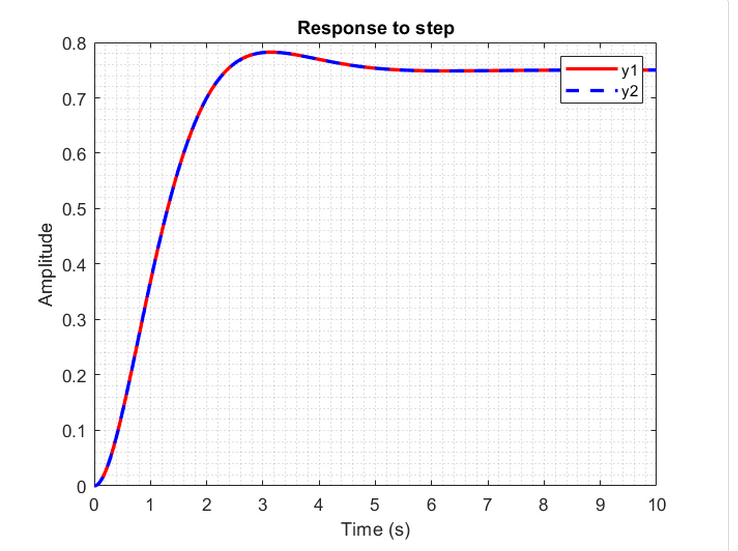
\includegraphics[width=15cm]{images/Q1_c_fig.png}
        \caption{Step Response}
        \label{fig:Q1c}
    \end{figure}

    We can tell from Fig.\ref{fig:Q1c} that the step responses are exactly the same.
    This make sense because we are representing the same system, and the output is the same for the two representations. 

\pagebreak
\section{Problem 2}
    Let \(\Sigma = \{0, 1\}\). Construct a DFA \(A\) that recognizes the
    language that consists of all binary numbers that can be divided by 5.
    
    \vspace{2mm}
    Let the state \(q_k\) indicate the remainder of \(k\) divided by 5. For
    example, the remainder of 2 would correlate to state \(q_2\) because \(7
    \mod 5 = 2\).

    \begin{figure}[h]
        \centering
        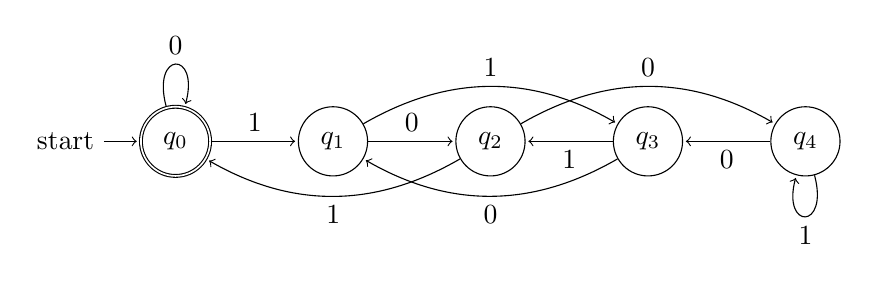
\begin{tikzpicture}[shorten >=1pt,node distance=2cm,on grid,auto]
            \node[state, accepting, initial] (q_0)   {$q_0$};
            \node[state] (q_1) [right=of q_0] {$q_1$};
            \node[state] (q_2) [right=of q_1] {$q_2$};
            \node[state] (q_3) [right=of q_2] {$q_3$};
            \node[state] (q_4) [right=of q_3] {$q_4$};
            \path[->]
                (q_0)
                    edge [loop above] node {0} (q_0)
                    edge node {1} (q_1)
                (q_1)
                    edge node {0} (q_2)
                    edge [bend right=-30] node {1} (q_3)
                (q_2)
                    edge [bend left] node {1} (q_0)
                    edge [bend right=-30] node {0} (q_4)
                (q_3)
                    edge node {1} (q_2)
                    edge [bend left] node {0} (q_1)
                (q_4)
                    edge node {0} (q_3)
                    edge [loop below] node {1} (q_4);
        \end{tikzpicture}
        \caption{DFA, \(A\), this is really beautiful, ya know?}
        \label{fig:multiple5}
    \end{figure}

    \subsection{Justification}

    Take a given binary number, \(x\). Since there are only two inputs to our
    state machine, \(x\) can either become \(x0\) or \(x1\). When a 0 comes
    into the state machine, it is the same as taking the binary number and
    multiplying it by two. When a 1 comes into the machine, it is the same as
    multiplying by two and adding one.

    Using this knowledge, we can construct a transition table that tell us
    where to go:

    \begin{table}[ht]
        \centering
        \begin{tabular}{c || c | c | c | c | c}
            & \(x \mod 5 = 0\)
            & \(x \mod 5 = 1\)
            & \(x \mod 5 = 2\)
            & \(x \mod 5 = 3\)
            & \(x \mod 5 = 4\)
            \\
            \hline
            \(x0\) & 0 & 2 & 4 & 1 & 3 \\
            \(x1\) & 1 & 3 & 0 & 2 & 4 \\
        \end{tabular}
    \end{table}

    Therefore on state \(q_0\) or (\(x \mod 5 = 0\)), a transition line should
    go to state \(q_0\) for the input 0 and a line should go to state \(q_1\)
    for input 1. Continuing this gives us the Figure~\ref{fig:multiple5}.

\pagebreak
\section{Problem 3}
    Write part of \alg{Quick-Sort($list, start, end$)}

    \begin{algorithm}
        \begin{algorithmic}[1]
            \Function{Quick-Sort}{$list, start, end$}
                \If{$start \geq end$}
                    \State{} \Return{}
                \EndIf{}
                \State{} $mid \gets \Call{Partition}{list, start, end}$
                \State{} \Call{Quick-Sort}{$list, start, mid - 1$}
                \State{} \Call{Quick-Sort}{$list, mid + 1, end$}
            \EndFunction{}
        \end{algorithmic}
        \caption{Start of QuickSort}
    \end{algorithm}

\pagebreak
\section{Problem 4}
\subsection{question}
\subsection{solution}
\pagebreak
\subsubsection{partA}

\pagebreak
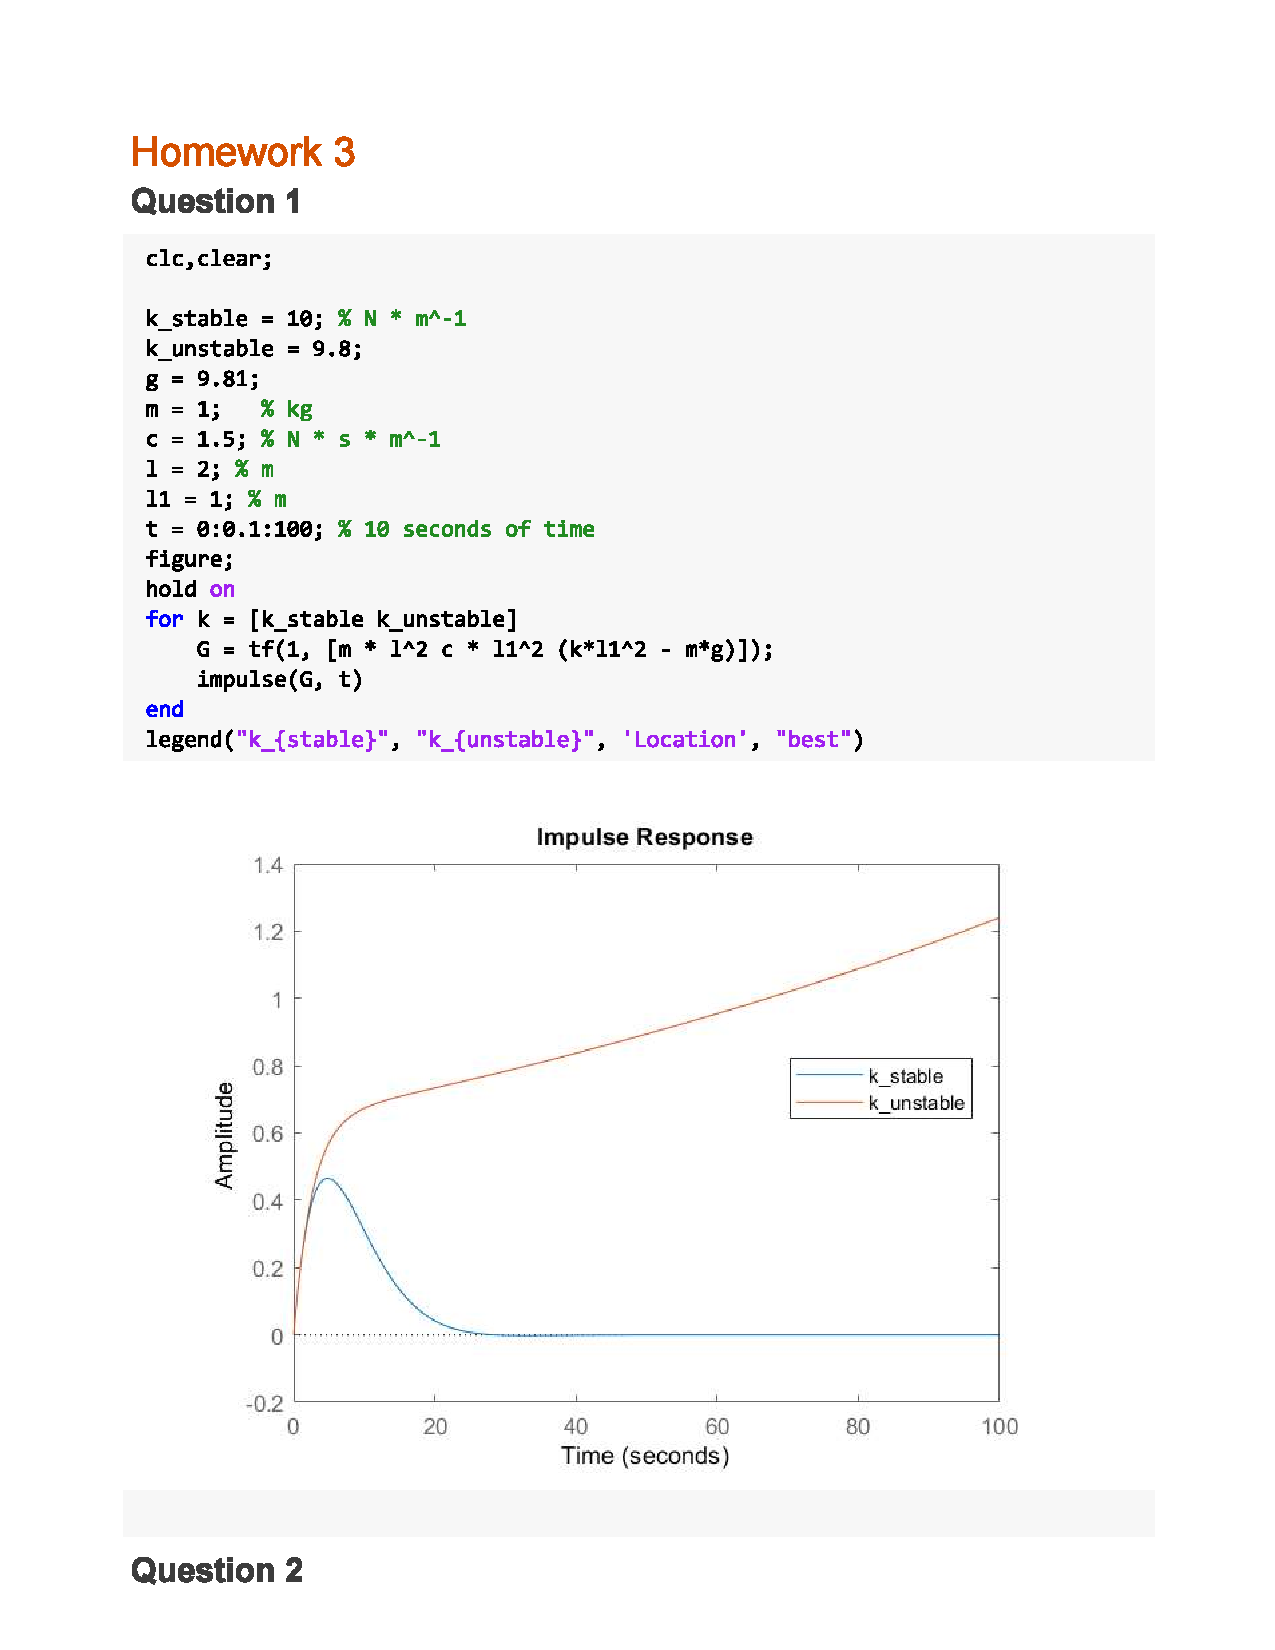
\includepdf{misc/matlab_p1.pdf}
% % Print the bibliography!
\printbibliography
\end{document}
